\documentclass[prd,twocolumn,showpacs,superscriptaddress,groupedaddress,nofootinbib]{revtex4}  % for review and submission
%\documentclass[aps,preprint,showpacs,superscriptaddress,groupedaddress]{revtex4}  % for double-spaced preprint
\usepackage{graphicx}  % needed for figures
%\usepackage[caption = false]{subfig}
\usepackage{lipsum}
\usepackage{dcolumn}   % needed for some tables
\usepackage{bm}        % for math
\usepackage{amsmath,amssymb}   % for math
\usepackage{aas_macros}
\usepackage{multirow}
\usepackage{color}
\usepackage{verbatim}
%\usepackage{times}
\usepackage{url}
\usepackage{hyperref}
\usepackage{csquotes}
\usepackage{natbib}
%\usepackage{subcaption}
% avoids incorrect hyphenation, added Nov/08 by SSR

\newcommand{\bs}{\boldsymbol}
\newcommand{\tcb}{\textcolor{blue}}
\newcommand{\tcr}{\textcolor{red}}
\newcommand{\Largr}{\mathcal{L}}

\hyphenation{ALPGEN}
\hyphenation{EVTGEN}
\hyphenation{PYTHIA}
\textheight=700pt
\begin{document}
% The following information is for internal review, please remove them for submission
\widetext
% the following line is for submission, including submission to the arXiv!!
%\hspace{5.2in} \mbox{Fermilab-Pub-04/xxx-E}
\title{Increasing Fisher Information using Moving-Mesh Reconstruction}
\author{Qiaoyin Pan}
\email{panda@mail.nankai.edu.cn}
\affiliation{School of Physics, Nankai University, 94 Weijin Rd, Nankai, Tianjin, 300071, China}
\affiliation{Canadian Institute for Theoretical Astrophysics, University of Toronto, 60 St. George Street, Toronto, Ontario M5S 3H8, Canada}
\author{Ue-Li Pen}
\email{pen@cita.utoronto.ca}
\affiliation{Canadian Institute for Theoretical Astrophysics, University of Toronto, 60 St. George Street, Toronto, Ontario M5S 3H8, Canada}
\affiliation{Dunlap Institute for Astronomy and Astrophysics, University of Toronto, Toronto, ON M5S 3H4, Canada}
\affiliation{Canadian Institute for Advanced Research, Program in Cosmology and Gravitation} 
\affiliation{Perimeter Institute for Theoretical Physics, Waterloo, ON, N2L 2Y5, Canada}
\author{Derek Inman}
\affiliation{Canadian Institute for Theoretical Astrophysics, University of Toronto, 60 St. George Street, Toronto, Ontario M5S 3H8, Canada}
\affiliation{Department of Physics, University of Toronto, 60 St. George, Toronto, ON M5S 1A7, Canada}
\author{Hao-Ran Yu}
\affiliation{Canadian Institute for Theoretical Astrophysics, University of Toronto, 60 St. George Street, Toronto, Ontario M5S 3H8, Canada}
\affiliation{Kavli Institute for Astronomy and Astrophysics, Peking University, Beijing 100871, China}

\date{\today}

\begin{abstract}
  Reconstruction techniques are commonly used in cosmology to reduce
  complicated nonlinear behaviours to a more tractable linearized
  system.  We study a new reconstruction technique that uses the
  Moving-Mesh algorithm to estimate the displacement field
  from nonlinear matter distribution. We show the performance of this
  new technique by quantifying its ability to reconstruct linear
  modes. We study the cumulative Fisher information $I(<k_n)$ about  
  the initial matter power spectrum in 130 $N$-body simulations before 
  and after reconstruction, and find that the nonlinear plateau of
  $I(<k_n)$ is increased by a factor of $\sim 50$ after reconstruction, from
  $I \simeq 2.5 \times 10^{-5} /({\rm Mpc}/h)^3$ to
  $I \simeq 1.3 \times 10^{-3}/({\rm Mpc}/h)^3$ at large $k$.
  This result includes the decorrelation between initial and final fields,
  which has been neglected in some previous studies.
We expect this technique to be
  beneficial to problems such as baryonic acoustic oscillations,
  redshift
space distortions and
  cosmic neutrinos that rely on accurately disentangling nonlinear
  evolution from underlying linear effects.
\end{abstract}


%\pacs{}
\maketitle

\begin{section}{Introduction}\label{sec:introduction}  

The power spectrum is widely used in modern cosmology to measure the matter
fluctuations. In the early universe, initial Gaussian density fields
can be completely described by the power spectrum, or the two-point
statistics. However, gravitational instability and nonlinear large scale
structure (LSS) formation make the matter distribution highly
non-Gaussian, and the galaxy distribution also follows this non-Gaussian
distribution. In these cases one needs to compute higher statistics
which are computationally more expensive and more difficult to
interpret into initial cosmological parameters. Fisher information
is usually used to quantify the amount of independent information
that is contained in the power spectrum estimation.

Rimes and Hamilton \citep{bib:Rimes2006} first study the Fisher
information contained in the matter power
spectrum given by $N$-body simulations, and find that there is a
plateau on translinear scales $(k \simeq 0.2-0.8\ h/{\rm Mpc})$,
which shows that on these scales, there is a strong coupling of
Fourier modes. Thus the power spectrum on smaller scales, gives little
additional independent information.

There are many approaches to recover the lost information in the
power spectrum of the matter density field, by transforming the final
density field into a more Gaussian, early stage density field.
For example, Gaussianization transforms are commonly used
\cite{bib:Weinberg1992,bib:Mark2009} to make the logarithmic
distribution more Gaussian. Nonlinear Wiener filters are used
in wavelet space to Gaussianize the fields and can also improve
the Fisher information \cite{bib:Zhang2011,bib:Yu2012,bib:HarnoisD2013}.
It is shown in \cite{bib:HarnoisD2013} that, although these methods
or their combinations may have different abilities to recover
the Fisher information, by means of reducing the mode coupling
and variances in the auto power spectrum of Gaussianized
density fields, they do not necessarily improve the cross correlation
 between the initial density
field and the final density field, and thus result in a smearing
out of the baryonic acoustic oscillations (BAO) peak in the two-point
correlation function. If one is concerned about mapping
the initial conditions to final conditions (e.g. measurement of 
BAO) these methods are unable to
extract valid information from initial conditions, at least in
the cross power spectrum between initial and final conditions.

Reconstruction techniques (including the one described in 
\cite{bib:HarnoisD2013}) are able to increase the Fisher information
while also improving the cross correlation with the initial conditions
and sharpening the BAO peak. It is based on the coupling of linear
density field $\delta_L(\bs{q},t_0)$ to the displacement field
$\bs\Psi(\bs{q})$ (first derived by \cite{bib:Zel1970}), which
is estimated by a smoothed final density field.
\cite{bib:Zhu2016} shows a new method in the estimation of displacement
field in 1-dimensional (1D), according to which the 1D linear density
field is reconstructed in Lagrangian space and successfully improves 
the BAO measurement. In 3D cases, it is nontrivial to estimate
the displacement field, but \cite{bib:Yu2016} shows that the displacement
field given by $N$-body simulations can be used to recover $\delta_L$.

In this paper we generalize the displacement field estimation method
from 1D \citep{bib:Zhu2016} to 3D, reconstruct $\delta_L$ and study
the Fisher information recovery in $\delta_L$. Here, the displacement field
estimation is done by a \textit{Moving-mesh} (MM) algorithm, which is based on
the \textit{Adaptive Particle-mesh} (APM) simulation algorithm \citep{bib:Pen1995,bib:Pen1998}.

This paper is organized as follows. 
In Section \ref{sec:reconstruction}, we briefly describe the reconstruction algorithm.
In Section \ref{sec:simulation}, we present the main steps of the $N$-body 
simulation code that are used to simulate the dark matter density fields, 
and the result of running the reconstruction code.
In Section \ref{sec:fisherinfo}, we calculate and compare the power spectra, 
correlation matrix and Fisher information given by simulation and reconstruction.
The discussion and conclusion are presented in Section \ref{sec:conclusion}

\end{section}


\begin{section}{Reconstruction Algorithm}
  \label{sec:reconstruction}
  
\tcb{Detailed description of MM algorithm can be found in
\cite{bib:ZhuH2016}. Here we quickly review it for completeness.}
The aim of the reconstruction is to estimate the Lagrangian position, or 
the displacement, of particles from their final position only. 
Due to the highly nonlinear process at the late stage, it is hard to 
fully discrible the displacement field from the final condition. 
However, since the result in \cite{bib:Yu2016} showed that the $E$-mode 
displacement field has a strong correlation with the linear density field 
on large scale ($r > 0.5$ when $k \lesssim 2 h/\mathrm{Mpc}$), estimating the 
$E$-mode displacement is expected to recover a large amount of information. 
It can be done by applying \textit{Moving-Mesh} (MM) algorithm discribed in 
\cite{bib:ZhuH2016}, which is originated from \textit{Adapting Particle-Mesh} 
(APM) algorithm \cite{bib:Pen1995,bib:Pen1998}.

The basic idea is to build a Particle-Mesh scheme on a curvilinear 
coordinate system, $\bm{\xi}=\left(\xi_1,\xi_2,\xi_3\right)$, in 
which number of particles per grid cell is set approximately constant. 
The displacement of particles in each grid cell is then approximately 
discribed by the deformation of the curvilinear grid on the Eulidean 
coordinate $\bm{x}(\bm{\xi},t)$.
Assuming that the deformation is a pure gradient, the physicsl position of 
particles on Eular coordinate is given as
\begin{align}
    x^i=\xi ^\mu \delta ^i _\mu + \Delta x^i,
\end{align}
where
\begin{align}
  \label{eq:disp}
    \Delta x^i=\frac{\partial \phi}{\partial \xi ^ \nu}\delta ^{i \nu} .
\end{align}
We use the convention the same as in \cite{bib:Pen1995}, Latin indices denoting 
Cartesian coordinate, while Greek indices denoting the curvilinear grid coordinate.
$\phi$ is called the deformation potential, and $\Delta x^i$ the lattice
displacement.
The coordinate transfromation matrix $e^i_\mu = \partial x^i / \partial \xi ^ \mu$
is guarantee to be positive definite so that the volume element 
$\sqrt{g} \equiv \mathrm{det}\left| e^i_\mu\right|$ is always positive. 
This choice of the deformation can minimize the cell-crossing.

To solve the deformation potential $\phi$, consider the continuity equation 
in curvilinear coordiante,
\begin{align}
 \label{eq:continue_eq}
    \frac{\partial (\sqrt{g} \rho) }{\partial t}+
    \partial_\mu \left[\rho \sqrt{g} e^\mu _i \left(v^i - 
    \Delta \dot{x}^i \right) \right] =0
\end{align}
$\Delta \dot{x}^i=\delta ^{i\nu}\partial _\nu \dot{\phi}$ is chosen such that the 
first term in Eq.\ref{eq:continue_eq} is zero, resulting in a constant mass 
per volume element. 
The velocity field divergence is replaced by the deviation density field 
$\Delta \rho = \bar{\rho}-\rho \sqrt{g}$, which ideally should be zero. 
Then the deformation potential is described via the elliptic equation,
\begin{align}
 \label{eq:li_elip}
    \partial _\mu (\rho \sqrt{g} e^\mu _i \delta^{i\nu}
    \partial_\nu \Delta \phi)=\Delta \rho.
\end{align}
The Eq.\ref{eq:li_elip} can be solved using multigrid algorithm described in 
\cite{bib:Pen1995,bib:Pen1998} (see also \cite{bib:ZhuH2016} for brief discription). 
The deformation $\Delta x^i$ is closer to the displacement of particles when 
higher resolution is used to decribed the density field so that less particles are 
contained in each grid cell.
\end{section}



\begin{section}{N-Body Simulations and Power Spectra}
  \label{sec:simulation}
  We use the \textsc{CUBEP$^3$M} code \cite{bib:Harnois2013} to run
  136 simulations with a box size of 300 Mpc/h and $512^3$ particles.
  The initial conditions are computed using the transfer function
  given by CAMB \cite{bib:Lewis2000} and then propagating the power
  back to $z=100$ with a linear growth factor.  The Zel'dovich
  approximation is used to calculate the displacement and velocity
  fields of the particles.  For these simulations, we use cosmological
  parameters $\Omega_M=0.321$, $\Omega_{\Lambda}=1.0-\Omega_m$,
  $h=0.67$, $\sigma_8=0.83$, and $n_s=0.96$.  Different random seeds
  are used to produce the initial conditions for different simulations
  so that they are independent of each other.

  \begin{figure}[h]
    \centering
    \includegraphics[width=0.45\textwidth]{fig1.pdf}
    \caption{ The 2-D projection of the deformed grid of a sample
      $N$-body simulations is shown as curved white lines.  The
      density fluctuation, $\delta\rho/\bar{\rho}$, is shown
      underneath.}
    \label{fig:simandrec}
 \end{figure}

  We use Cloud-In-Cell (CIC) interpolation to estimate the density
  contrast $\delta_S=\delta\rho/\rho-1$ from the particles.  We then
  apply the MM reconstruction to these fields with a resolution of
  $128^3$ cells.  A 2D projection of the deformed grids and the
  original density field are given in Fig. \ref{fig:simandrec}.  As
  expected, there is no grid crossing after reconstruction.
 
 The cross power spectrum, $P_{ij}(k)$, is defined as
 \begin{align}
   \langle \delta_i \left( \bm{k} \right) \delta_j \left( \bm{k'}\right) \rangle =
   \left( 2\pi \right) ^3 P_{ij} \left( k \right) \delta_D \left( \bm{k}-\bm{k'} \right),
 \end{align}
 where $\delta_{i}$ and $\delta_j$ are density contrasts and
 $\delta_D$ is the Dirac delta funciton. We typically consider instead
 the dimensionless power spectrum, $\Delta_{ij}^2(k)$, defined as
 \begin{align}
   \Delta_{ij}^2(k) \equiv \frac{k^3 P_{ij} \left( k \right)}{2\pi ^2}.
 \end{align}
 In the left panel of Fig. \ref{fig:cp}, we show the matter auto power spectrum
 ($i=j$) of linear theory density fields ($\delta_L$), from the
 simulation results ($\delta_S$) and after reconstruction
 ($\delta_R=-\nabla^2\phi$).  For the simulation and reconstruction
 results, we use the average value of all 136 simulations and show
 $1\sigma$ variances as error bars.  To determine the correlation
 between fields, we compute the cross correlation coefficient
 $r_{ij}(k) = P_{ij}/\sqrt{P_{ii}P_{jj}}$.  In the right panel of Fig. \ref{fig:cp}(b),
 we show $r_{SL}$ and $r_{RL}$.  We see that the reconstructed field
 is much more highly correlated with the linear field than the
 simulation field is.  Specifically, we find that the scale at which
 $r(k)=1/2$ drops from $k\simeq $0.2 h/Mpc to $0.6 $h/Mpc.  In
 comparison with the results of \citet{bib:ZhuH2016}, we find the
 correlation coefficient falls off at slightly lower wavenumbers which
 we attribute to using lower resolution simulations.

  \begin{figure*}
    \centering
    \includegraphics[width=0.48\textwidth]{fig2b.pdf}
    \includegraphics[width=0.455\textwidth]{fig2a.pdf}
    \caption{{\it Left.} The dimensionless power spectrum computed via
      linear theory (black), the mean value of 136 $N$-body
      simulations with $1\sigma$ error bars (blue), and reconstruction
      of the simulations (red).  {\it Right.} The cross correlation
      function (solid lines) $r_{\delta\delta_L}$ (blue) and
      $r_{\delta_R\delta_L}$ (red), and BAO damping models (dash
      lines).}
    \label{fig:cp}
  \end{figure*}


\end{section}



\begin{section}{Power Spectra and Information Content}
  \label{sec:fisherinfo}
    The power spectrum is the Fourier transform of the correlation function and measures the amoutn of clustering in the matter distribution in terms of the wavenumber $k$ in unit of $h \mathrm{Mpc}^{-1}$,
\begin{align}
    \langle \delta \left( \bm{k} \right) \delta \left( \bm{k'}\right) \rangle =\left( 2\pi \right) ^3 P \left( \bm{k} \right) \hat{\delta} \left( \bm{k}-\bm{k'} \right),
\end{align}
where $\delta \left( \bm{k} \right)$ is the density fluctuation in wave space, while $\hat{\delta}$ is the delta funciton. Of equal interest is $\Delta ^2_k$, the power spectrum in its dimensionless form, defined as
\begin{align}
    \Delta ^2_k \equiv \frac{k^3 P \left( k \right)}{2\pi ^2}
\end{align}
    The power spectra of the mass distributions are calculated using the "Nearest Grid Point" (NGP) mass assignment scheme, which calculates the position of each particle based on which grid point it is nearest. In Fig.... we plot the mean power spectrum (and error bars) of 139 density fields and reconstruced deformation potentials.
    To calculate the cumulative Fisher information of the density fields, the covariance matrix of the power spectra should be first given. Mathematically, the the covariance matrix is defined as
\begin{align}
    \mathrm{Cov}\left(k,k'\right)\equiv \frac{1}{N-1}\sum_{i=1}^{N}\left[ P_i \left( k \right) - \langle P \left( k \right) \rangle \right]\left[ P_j \left( k' \right) - \langle P \left( k' \right)\rangle \right],
\end{align}
where angle brackets mean the expected values. 
    The cross-correlation coefficient matrix, or for short, the correlation matrix, is a normalized version of the covariance matrix,
\begin{align}
    \mathrm{Corr}\left(k,k'\right)=\frac{\mathrm{Cov}\left(k,k'\right)}{\sqrt{\mathrm{Cov}\left(k,k\right)\mathrm{Cov}\left(k',k'\right)}}.
\end{align}
The corelation matrices for density fields from simulations and deformation potentials from reconstructions are shown in Fig. \ref{fig:corrall}. For the original density fields, the linear regime, where $k<0.1$, is diagonal, while in the non-linear regime, the power spectra of different $k$ modes are strongly correlated by at least $60\%$ . For the reconstructed deformation potential correlation matrix, however, the linear regime expand up to $k~0.2$. The correlation matrix is closer to that for the power spectra of linear density fields.
\begin{figure}
 \centering
% \begin{subfigure*}[b]{0.5\textwidth}
% \centering
  \includegraphics[width=0.5\textwidth]{corr2-crop.pdf}
%\label{fig:corrnb}
% \end{subfigure*}
% \begin{subfigure*}[b]{0.5\textwidth}
% \centering
%  \includegraphics[width=0.45\textwidth]{corrrecnew-crop.pdf}
%\label{fig:corrrec}
% \end{subfigure*}
%\begin{subfigure}
%\begin{figure}
%  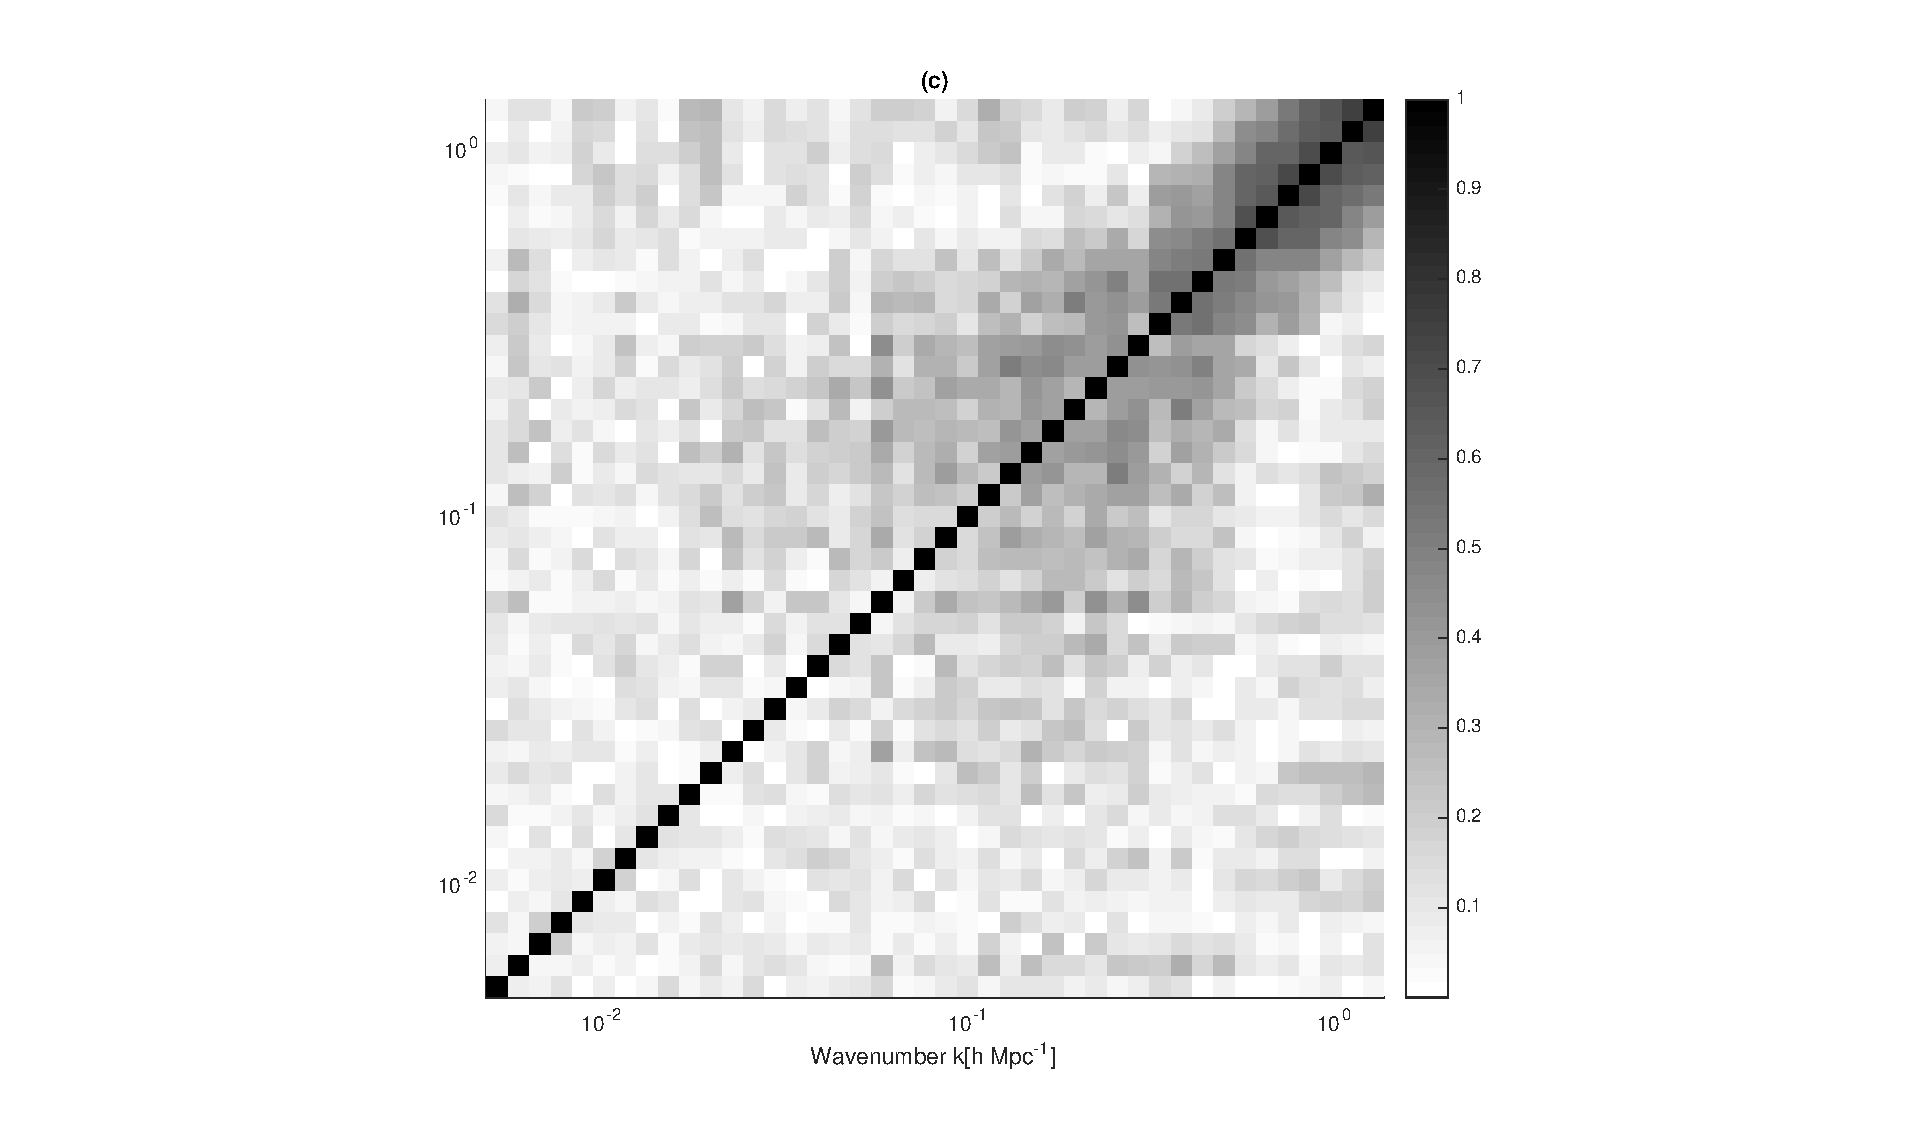
\includegraphics[width=0.5\textwidth]{corrlin.eps}
% \end{subfigure}
%\begin{figure}
%    \centering
%    \includegraphics[width=\textwidth,height=0.5\textwidth]{corrall.eps}
%
  \caption{Cross-correlation coefficient matrix as found from 136 power spectra of the non-linear density field from simulation (the upper triangle) and the deformation potential field from reconstruction(the lower triangle).}   

    \label{fig:corrall}
\end{figure}
    The cumulative, or Fisher, information function of $k_n$ is then defined as the sum of the elements of inverse of subsection of the normalized covariance matrix up to $k_n$ scale
\begin{align}
    I \left( < k_n\right) = \sum_{i,j=1}^n \left[ C^{-1}_{norm} \left( k_i,k_j \right)\right] \left( i,j \leq n \right),
\end{align}
where $C_{norm}$ is the normalized covariance matrix, defined as
\begin{align}
    C_{norm} \left( k,k' \right)=\frac{\mathrm{Cov}(k,k')}{\langle P(k)\rangle\langle P(k)\rangle}.
\end{align}
  
%  The signal-to-noise ratio, sometimes also called Fisher information, can be given by the inverse matrix of covariance. Since the signal-to-noise ratio was given in some work, we also present it for a better comparison. 
%\begin{align}
%\left( \frac{S}{N}\right)^2 (k_{n}) =\sum_{i,j=1}^n P_i \mathrm{Cov}^{-1}(i,j) P_j
%\end{align}
As seen above, cumulative information is a measurement of the number of independent Fourier modes presented in a field up to a given $k_n$, which represents how linear a field is. We plot the cumulative information of the power specta of density fields from simulations and deformation potentials from reconstructions in Fig.\ref{fig:fisherinfo}. In the translinear regime, where $k\sim0.1$, the cumulative information of the non-linear density field has a flat plateau. It indicates that there's nearly no independent information in the translinear regime of the power spectrum. At $k\sim0.8$, the information increase slightly aggain. But the information curve of the reconstructed deformation potential keeps incresing and reaches it's plateau at $k\sim0.6-0.7$ up to a factor of 20. It indicates that APM method can strongly recover the lost information within this scale. 
\begin{figure}[htbp]
 \begin{center}
  \includegraphics[width=0.5\textwidth]{fishernew-crop.pdf}
   \caption{Cumulative information in the power spectra as a function of wavenumber. The blue cycles correspond to the non-linear density field by simulation; the black squares correspond to the the reconstructed deformation potential; the red dash line corresponds to linear density field at $z=0$; the green crosses correspond to linear density field at $z=100$.}
  \label{fig:fisherinfo}
 \end{center}
\end{figure}


\end{section}


\begin{section}{Conclusion and Discussion}
 \label{sec:conclusion}
    We use the code "CubeP3M" to generate 136 independent dark matter density fields, 
then give the reconstructed deformation potentials which are pure divergent using MM 
algorithm. We analyze the power spectra of both the non-linear density fields and 
reconstructed density fields, after which we give the cross correlation matrix. We find that the power 
spectra are highly correlated on small scales, since these scales are in non-linear 
regime. But after reconstruction, the strongly correlated regime shinks from $k\sim0.2$ 
to $k\sim0.6$. We also calculate the cumulative information, and find that the plateau 
of the reconstructed information curve keeps matching the Gausisan information curve until 
$k \sim 0.3$ and reach a plateau at $k \sim 0.8$, rising by a factor of 40 compared to the 
non-linear information curve.

   We argue that the reconstructed Fisher information will still increasing to a greater magnitude in smaller scale 
since the cross correlation of the reconstructed and linear power spectrum increases 
in a higher resolution analysis cite(bib:ZhuH2016).

   The new reconstruction method successfully recovers the lost linear information on 
the mildly non-linear scale, better than previous methods 
\cite{bib:Mark2006,bib:Mark2009,bib:Zhang2011,bib:Yu2012,bib:Mark2014} and pushes the 
non-linear scale to a smaller scale in our case. The result in dark matter density fields 
gives a strong motivation to adapt MM reconstruction in halo fields, neutrino fields, etc, so that 
we have access to know more clearly about the physics in smaller scale. Some efforts were 
made to improve cosmology measurements to BAO scale (e.g. \cite{bib:Daniel2007,bib:Martin2015}). 
MM reconstruction gives the reconstructed displacement given on the Lagrangian coordinates transfromed from the 
Eulerian coordiantes. It's successful try on BAO reconstruction in 1-D 
\cite{bib:Zhu2016} and 3-D cite(bib:ZhuH2016) cosmology provided an intuitive view of the algorithm 
to push forward the BAO research.

   MM reconstruction effectively decomposes the irrotational part and the curl part of the displacement 
field of particles.
On the other hand, the reconstructed displacement might be greatly different from real displacement in N-body 
simulation, since it's sensitive to the late stage shell-crossing and non-linear process so that the original 
position of some spectific particles can be replaced by each other. It's meaningful to compare the irrotational 
displacement field through MM reocnstruction and that from E-mode displacement reconstruction \cite{bib:Yu2016} 
which decomposes cleanly the irrotational and curl part of the real displacement in N-body simulation. 
Since MM reconstruction only needs the density field input and gives a latge recovering of lost information, 
it's expected to have a good effect on reconstructing the matter density field from obsurvation.
\end{section}


\acknowledgements{
  \label{sec:acknowledgements}
  We thank Homg-Ming Zhu and Wang Xin for friendly and helpful discussion.  Computations were performed on
  the General Purpose Cluster supercomputer at the SciNet HPC
  Consortium.  SciNet is funded by: the Canadian Foundation for
  Innovation under the auspices of Compute Canada; the Government of
  Ontario; Ontario Research Fund - Research Excellence; and the
  University of Toronto.  
}


\bibliographystyle{apsrev}
\bibliography{myreference}

\end{document}
